\section{Η αρχιτεκτονική BOOM (2011) ΕΕ}


% ------------------------------------------------------------------------------------------
% The  BOOM  Project:  Towards  160  Gb/s  Packet Switching  Using  SOI  Photonic  Integrated
% Circuits  and  Hybrid  Integrated  Optical Flip-Flops
% ------------------------------------------------------------------------------------------

Tο ευρωπαϊκό έργο BOOM επιχειρεί την ανάπτυξη μιας πλατφόρμας
φωτονικής δρομολόγησης, βασιζόμενης σε υβριδικά silicon-on-insulator
(SOI) integrated PICs, για την υλοποίηση όλων των λειτουργιών
δρομολόγησης, όπως είναι η ανίχνευση ετικετών, η παραγωγή σήματος
ελέγχου, η μετατροπή μήκους κύματος (WC: wavelength conversion) και η
εναλλαγή μήκους κύματος (WS: wavelength switching).

Ο συγχρονισμός πακέτων μπορεί να πραγματοποιηθεί χρησιμοποιώντας
οπτικά buffers βασισμένα σε delay lines \cite{5685653}, ή στοιχεία
βοηθούμενα από micro-resonators. Τα υβριδικά στοιχεία υλοποιούνται με
τεχνικές flip-chip bonding και heterogenous wafer scale integration.
Αυτές επιτρέπουν τη δημιουργία στοιχείων όπως είναι οι ultra-fast
all-optical wavelength converters, λέιζερ ηλεκτροαπορρόφησης (EML:
electroabsorption-modulated lasers), WDM φωτοανιχνευτές και microring
resonator (ΜΡΡ) based διασυνδέσεις σε επιστρώματα πυριτίου.

H αρχιτεκτονική BOOM έχει σύγχρονισμένη εισαγωγή labeled πακέτων σε
διαφορετικά μήκη κύματος. Η διαδικασία μεταγωγής αρχίζει με πακέτα που
φθάνουν στον κόμβο σε προκαθορισμένες χρονικές θυρίδες και
χρησιμοποιούνται τρία υποσυστήματα για τη δρομολόγηση των πακέτων.  Το
πρώτο εκτελεί ανίχνευση ετικετών μέσω ultra-dense wavelength division
(UDWDM) αποδιαμρφωτών που φιλτράρουν τις οπτικές ετικέτες. Ο
αποδιαμορφωτής UDWDM περιλαμβάνει συμπαγείς MRRs και συστοιχίες
ενσωματωμένων ανιχνευτών κατασκευασμένων σε SOI μέσω τεχνικών die-to
wafer bonding.

Τα παραγόμενα ηλεκτρικά σήματα στη συνέχεια παρέχονται για περαιτέρω
ηλεκτρονική επεξεργασία.  Ο ηλεκτρονικός επεξεργαστής -που μπορεί να
είναι τυπικά ένα FPGA- παράγει το σήμα ελέγχου που οδηγεί το
all-optical wavelength converter υποσύστημα. Το τελευταίο περιλαμβάνει
EMLs και high-speed AOWCs flip-chip integrated στην ίδια SOI
πλατφόρμα. Τα EMLs έπιτελούν τη μετατροπή από ηλεκτρικό σε οπτικό σήμα
(E/O conversion).

Τα οπτικά σήματα οδηγούνται σε ενσωματωμένους υβριδικούς WCs,
αλλάζοντας τα μήκη κύματος των εισερχομένων πακέτων δεδομένων και
βοηθώντας τη διαδικασία δρομολόγησης.

Οι ultra-fast AOWCs αποτελούνται από InP semiconductor optical
amplifiers (SOAs) και από ένα ζεύγος κασκοδικών SOI DIs. Οι SOAs
εκτελούν cross gain και phase modulation, ενώ τα κασκοδικά
συμβολόμετρα χρησιμοποιούνται για chirp filtering και αναστροφή
πολικότητας. Αυτός ο τύπος μετατροπής μήκους κύματος έχει επιδειχθεί
με εξαρτήματα διακριτών στοιχείων για datarates πέραν των 160 Gb/s
\cite{5295346}

Στην εικόνα \ref{fig:boom}, φαίνεται η αρχιτεκτονική δρομολόγησης
BOOM, χρησιμοποιώντας ένα 4x4 wavelength-based cross-connect με 2-D
grids από΄SOI MRRs. Σύμφωνα με το μήκος κύματος των ετικετών,
ενεργοποιείται ένα διαφορετικό σύμπλεγμα από φωτοανιχνευτών, EML και
μετατροπέων μήκους κύματος, αλλάζοντας το χρώμα των αρχικών ροών
πακέτων. Τα πακέτα αλλαγμένου μήκους κύματος εισέρχονται στο 4x4
switching matrix και δρομολογούνται σε συγκεκριμένες εξόδους ανάλογα
με το νέο χρώμα του μήκους κύματός τους. Ολόκληρο το σύστημα
δρομολόγησης μπορεί να υποστηρίξει ταχύτητες γραμμών 160 Gb / s, με
κατανάλωση ισχύος καθοριζόμενη κυρίως από τα στάδια μετατροπής των
μηκών κύματος.

\begin{figure}[h]
  \centering
  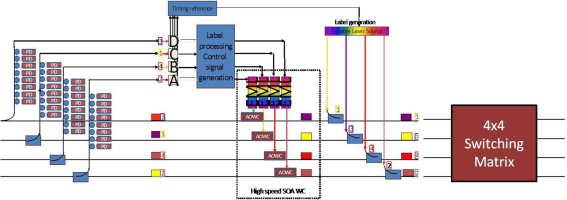
\includegraphics[width=.7\linewidth]{boom.png}
  \caption{Αρχιτεκτονική δρομολόγησης του ΒΟΟΜ}
  \label{fig:boom}
\end{figure}

Η πλατφόρμα που χρησιμοποιεί η αρχιτεκτονική BOOM απαιτεί τη
συγκέντρωση υβριδικών εξαρτημάτων για τη συναρμολόγηση και την
αξιολόγησή της. Δεδομένης όμως της διαθεσιμότητας μιας ποικιλίας
παθητικών δομών που μπορούν εύκολα να διασυνδεθούν με εμπορικά ενεργά
στοιχεία, θα ήταν δυνατόν να σχεδιαστεί μια ελαφρώς τροποποιημένη
αρχιτεκτονική δρομολόγησης, βασισμένη σε all-optical επεξεργασία
σήματος των ετικετών και των πακέτων δεδομένων. Η εικόνα \ref{fig:boom2}
δείχνει το all-optical κύκλωμα που εκτελεί packet switching με MRRs,
all-optical flip/flops και ultra-fast wavelength converters.

\begin{figure}[h]
  \centering
  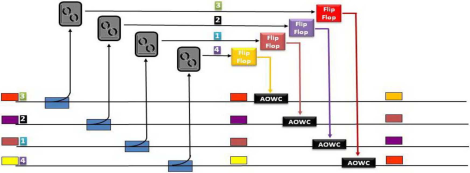
\includegraphics[width=.7\linewidth]{boom2.png}
  \caption{Σχεδιάγραμμα οπτικής μεταγωγής του BOOM}
  \label{fig:boom2}
\end{figure}

%%% Local Variables:
%%% mode: latex
%%% TeX-master: "main"
%%% TeX-engine: xetex
%%% End:
